\newpage



\appendix

\begin{widetext}
\section{NLO QED corrections in APFEL} \label{sec:appendixAPFEL}

In this section we discuss the details of the implementation of the
NLO QCD+QED corrections in {\tt APFEL}. While the inclusion of the LO
QED corrections presents many simplifications, $e.g.$ QED and QCD
corrections do not mix and thus the DGLAP equations as well as the
$\alpha_s$ and $\alpha$ evolution equations are decoupled, when going
to NLO, QED and QCD contributions mix both in the DGLAP and in the
coupling evolution equations. On top of this, such corrections induce
the presence of diagrams in which a real photon is present either in
the initial or in the final state and that have to be included in the
computation of the DIS structure functions. In the following we will
first discuss how to generalize the coupling evolution equations
(finding that the presence of the mixed QCD+QED terms leads to a
negligible difference in the running), we will then turn to the DGLAP,
and finally we will consider both Neutral-Current (NC) and
Charged-Current (CC) DIS structure functions.

\subsection{Evolution of the couplings}

As already mentioned, NLO QCD+QED corrections induce the presence of
mixed termsAt the level of the couplings, this essentially means that
the QCD $\beta$-function will get corrections proportional to $\alpha$
and, vice-versa, the QED $\beta$-function will get corrections
proportional to $\alpha_s$, in such a way that the coupling evolution
equations read:
\begin{equation}\label{CoupledEq}
\begin{array}{rcl}
\displaystyle \mu^2\frac{\partial \alpha_s}{\partial \mu^2} &=& \displaystyle
                                                \beta^{\rm QCD}(\alpha_s,\alpha)\,.\\
\\
\displaystyle \mu^2\frac{\partial \alpha}{\partial \mu^2} &=& \displaystyle \beta^{\rm QED}(\alpha_s,\alpha)\,.
\end{array}
\end{equation}
As a consequence, these evolution equations form a set of coupled
differential equations. Up to three loops ($i.e.$ NLO), the
$\beta$-functions can be expanded as:
\begin{equation}
\beta^{\rm QCD}(\alpha_s,\alpha) = -\alpha_s\left[\beta_0^{(\alpha_s)}\left(\frac{\alpha_s}{4\pi}\right)+\beta_1^{(\alpha_s\alpha)}\left(\frac{\alpha_s}{4\pi}\right) \left(\frac{\alpha}{4\pi}\right)+\beta_1^{(\alpha_s^2)}\left(\frac{\alpha_s}{4\pi}\right)^2+\dots\right]\,,
\end{equation}
and:
\begin{equation}
\beta^{\rm QED}(\alpha_s,\alpha) = -\alpha\left[\beta_0^{(\alpha)}\left(\frac{\alpha}{4\pi}\right)+\beta_1^{(\alpha\alpha_s)}\left(\frac{\alpha}{4\pi}\right) \left(\frac{\alpha_s}{4\pi}\right)+\beta_1^{(\alpha^2)}\left(\frac{\alpha}{4\pi}\right)^2+\dots\right]\,,
\end{equation}
where the ``new'' terms are the mixing terms
$\beta_1^{(\alpha_s\alpha)}$ and $\beta_1^{(\alpha\alpha_s)}$, and the
pure NLO QED term $\beta_1^{(\alpha^2)}$ have been computed in
Ref.~\cite{Surguladze:1996hx}. Taking into account a factor four due
the different definitions of the expansion parameter and writing
explicitly the color factors one finds:
\begin{equation}\label{eq:NewBetaTerms}
\beta_1^{(\alpha_s\alpha)} = -2\sum_{i=1}^{n_f}
e_q^2\,\qquad\beta_1^{(\alpha\alpha_s)} = -\frac{16}{3}N_c\sum_{i=1}^{n_f} e_q^2\,,\qquad \beta_1^{(\alpha^2)} = -4\left(n_l+N_c\sum_{i=1}^{n_f} e_q^2\right)\,.
\end{equation}
where $N_c=3$ is the number of colors, $e_q$ is the electric charge of
the quark flavour $q$, and $n_f$ and $n_l$ are the numbers of active
quark and leptons flavours, respectively.


Eq.~(\ref{CoupledEq}) can be written in the vectorial form:
\begin{equation}\label{CoupledEqVect}
\mu^2\frac{\partial {\bm \alpha}}{\partial \mu^2} = {\bm \beta}\left({\bm \alpha}(t)\right)\,,
\end{equation}
with:
\begin{equation}
  {\bm \alpha} = {\alpha_s \choose \alpha}\qquad\mbox{and}\qquad  {\bm \beta} = {\beta^{\rm QCD} \choose \beta^{\rm QED}}\,.
\end{equation}
Eq.~(\ref{CoupledEqVect}) is an Ordinary Differential Equation that
can be numerically solved using the Runge-Kutta method.

The first two terms in eq.~(\ref{eq:NewBetaTerms}) are repsonsible for
the coupling of the evolution of $\alpha_s$ and $\alpha$ and thus they
introduce a complication that affects both the implementation and the
performance of the relative code. One can then ask what is the effect
of their presence and whether their removal makes a substantial
difference. In Fig.~\ref{fig:CouplingEvol} we show the comparison
between the evolution at NLO of both couplings $\alpha_s$ and $\alpha$
including and excluding the mixing terms in the respective
$\beta$-functions. The evolution is performed between the $Z$ mass
scale $M_Z$ and 10 TeV with 5 active quark flavours and 3 active
lepton flavours and uses as boundary conditions
$\alpha_s(M_Z) = 0.118$ and $\alpha(M_Z) = 1/128$. The two curves in
Fig.~\ref{fig:CouplingEvol} are normalized to the respective curve
without mixing terms. It is clear that the mixed terms lead to tiny
relative differences that are at most of $\mathcal{O}(10^{-4})$ at 10
TeV for $\alpha_s$ and $\mathcal{O}(10^{-3})$ at the same scale for
$\alpha$. We conclude that the mixed terms in the $\beta$-functions
have a negligible effect on the coupling evolution and thus we exclude
them to make the code simpler and improve the performance without
introducing any significant inaccuracy.

%%%%%%%%%%%%%%%%%%%%%%%%%%%%%%%%%%%%%%%%%%%%%%%%%%%%%%%%
\begin{figure}[h]
\includegraphics[width=6cm,angle=270]{figs/couplings.eps} 
\caption{Comparison between the evolution of the QCD and QED couplings
  $\alpha_s$ and $\alpha$ including and excluding the mixed terms in
  the respective $\beta$-functions. The curves are normalized to the
  evolution without mixing terms.}
\label{fig:CouplingEvol}
\end{figure}
%%%%%%%%%%%%%%%%%%%%%%%%%%%%%%%%%%%%%%%%%%%%%%%%%%%%%%%%

\subsection{Evolution of the PDFs}

In this section we address the question of implementing the full NLO
QCD+QED corrections to the DGLAP evolution equations. Here we limit
ourselves to consider only the photon PDF without including the
leptons. The generalization to the full set of PDFs can be achieved
realtively easily following the same steps discussed below.

The first step towards an efficient implementation of the solution of
the DGLAP equations in the presence of QED corrections is the adoption
of a suitable set of combinations of PDFs that diagonalize the
splitting function matrix, decoupling as many DGLAP equations as
possible. Such a set of combinations (or basis) was already introduced
in Appendix A of Ref.~\cite{Bertone:2015lqa} and will be used also
here (without considering the distributions involving leptons). The
basis reads:
\begin{equation}\label{eq:EvolBasis}
\begin{array}{ll}
\mbox{\texttt{ 1} : }g & \\
\mbox{\texttt{ 2} : }\gamma & \\
\mbox{\texttt{ 3} : }\displaystyle \Sigma = \Sigma_u + \Sigma_d & \quad
\mbox{\texttt{9} : }\displaystyle V =V_u +  V_d\\
\mbox{\texttt{ 4} : } \displaystyle \Delta_\Sigma = \Sigma_u - \Sigma_d& \quad\displaystyle 
\mbox{\texttt{10} : } \Delta_V = V_u - V_d\\
\mbox{\texttt{ 5} : }T_1^u = u^+ - c^+ &\quad \mbox{\texttt{11} : }V_1^u = u^- - c^- \\
\mbox{\texttt{ 6} : }T_2^u = u^+ + c^+ - 2t^+ &\quad \mbox{\texttt{12} : }V_2^u = u^- + c^- - 2t^-\\
\mbox{\texttt{ 7} : }T_1^d = d^+ - s^+ &\quad \mbox{\texttt{13} : }V_1^d = d^- - s^- \\
\mbox{\texttt{ 8} : }T_2^d = d^+ + s^+ - 2b^+ &\quad \mbox{\texttt{14}
                                               : }V_2^d = d^- + s^- -
                                               2b^-\\
\end{array}
\end{equation}
where we have defined $q^\pm = q\pm\overline{q}$ with
$q = u,d,s,c,b,t$ and:
\begin{equation}
\begin{array}{ll}
\Sigma_u = u^++c^++t^+, &\quad V_u = u^-+c^-+t^-,\\
\\
\Sigma_d = d^++s^++b^+,&\quad V_d = d^-+s^-+b^-\,.
\end{array}
\end{equation}
The second step is construct the splitting function matrix responsible
for the evolution of each one of the distributions defined above. To
do so, we split each splitting function $P$ into a pure QCD term
$\widetilde{P}$, which only depends on $\alpha_s$, and a QCD+QED
correction term $\bar{P}$, which instead contains contributions having
at least one power of $\alpha$ but that can also contain mixed
terms. In practice:
\begin{equation}
P = \widetilde{P} + \bar{P}\,,
\end{equation}
where:
\begin{equation}\label{eq:PureQCDSplittings}
\widetilde{P} = \alpha_s \mathcal{P}^{(1,0)} + \alpha_s^2 \mathcal{P}^{(2,0)}+\dots\,,
\end{equation}
and:
\begin{equation}\label{eq:QCD+QEDSplittings}
\bar{P} = \alpha \mathcal{P}^{(0,1)} + \alpha_s\alpha \mathcal{P}^{(1,1)}+\alpha^2 \mathcal{P}^{(0,2)}\dots
\end{equation}
Note that in the r.h.s. of both eqs.~(\ref{eq:PureQCDSplittings})
and~(\ref{eq:QCD+QEDSplittings}) we are using the notation of
Refs.~\cite{deFlorian:2015ujt,deFlorian:2016gvk} to indicate the power
of $\alpha_s$ and $\alpha$ that a given splitting function multiplies.

The structure of the pure QCD splitting function matrix
$\widetilde{P}$ as well as the first term in $\bar{P}$, which
represents the LO QED correction, in the basis given in
eq.~(\ref{eq:EvolBasis}) was discussed in
Ref.~\cite{Bertone:2015lqa}. It is now necessary to analyze the
structure of the two additional terms $\mathcal{P}^{(1,1)}$ and
$\mathcal{P}^{(0,2)}$. Let us start we the
$\mathcal{O}(\alpha_s\alpha)$ correction. The resulting evolution
equations at this order are:
\begin{equation}
\begin{array}{rcl}
\displaystyle\left.\mu^2\frac{\partial}{\partial \mu^2}
\begin{pmatrix}
g\\
\gamma\\
\Sigma\\
\Delta_\Sigma
\end{pmatrix}
\right|_{\mathcal{O}(\alpha_s \alpha)} &=& \displaystyle \begin{pmatrix}
e_\Sigma^2 \mathcal{P}^{(1,1)}_{gg}      & e_\Sigma^2 \mathcal{P}^{(1,1)}_{g\gamma} & \eta^+\mathcal{P}^{(1,1)}_{gq} & \eta^-\mathcal{P}^{(1,1)}_{gq} \\
e_\Sigma^2 \mathcal{P}^{(1,1)}_{\gamma g} & e_\Sigma^2 \mathcal{P}^{(1,1)}_{\gamma\gamma} & \eta^+\mathcal{P}^{(1,1)}_{\gamma q} &\eta^-\mathcal{P}^{(1,1)}_{\gamma q} \\
2 e_\Sigma^2 \mathcal{P}^{(1,1)}_{qg}    & 2 e_\Sigma^2 \mathcal{P}^{(1,1)}_{q\gamma} & \eta^+\mathcal{P}^{+(1,1)}  & \eta^-\mathcal{P}^{+(1,1)}\\
2 \delta_e^2 \mathcal{P}^{(1,1)}_{qg} & 2 \delta_e^2 \mathcal{P}^{(1,1)}_{q\gamma} &\eta^-\mathcal{P}^{+(1,1)} &\eta^+\mathcal{P}^{+(1,1)}
\end{pmatrix}\otimes
\begin{pmatrix}
g\\
\gamma\\
\Sigma\\
\Delta_\Sigma
\end{pmatrix}
\end{array}\,,
\end{equation}

\begin{equation}
\displaystyle\left.\mu^2\frac{\partial}{\partial \mu^2}
\begin{pmatrix}
V\\
\Delta_V
\end{pmatrix} \right|_{\mathcal{O}(\alpha_s \alpha)}= 
\begin{pmatrix}
\eta^+\mathcal{P}^{-(1,1)} & \eta^-\mathcal{P}^{-(1,1)} \\
\eta^-\mathcal{P}^{-(1,1)} & \eta^+\mathcal{P}^{-(1,1)} 
\end{pmatrix}\otimes
\begin{pmatrix}
V\\
\Delta_V
\end{pmatrix}\,,
\end{equation}

\begin{equation}
\begin{array}{ll}
\begin{array}{rcl}
\displaystyle \left.\mu^2\frac{\partial T^u_{1,2}}{\partial \mu^2}\right|_{\mathcal{O}(\alpha_s \alpha)} &=&
\displaystyle e_u^2\mathcal{P}^{+(1,1)}\otimes T^u_{1,2}
\end{array}\,, &
\begin{array}{rcl}
\displaystyle \left.\mu^2\frac{\partial T^d_{1,2}}{\partial \mu^2}\right|_{\mathcal{O}(\alpha_s \alpha)} &=&
\displaystyle e_d^2\mathcal{P}^{+(1,1)} \otimes T^d_{1,2}
\end{array}\,,
\\
\\
\begin{array}{rcl}
\displaystyle \left.\mu^2\frac{\partial V^u_{1,2}}{\partial \mu^2}\right|_{\mathcal{O}(\alpha_s \alpha)} &=&
\displaystyle e_u^2\mathcal{P}^{-(1,1)} \otimes V^u_{1,2}
\end{array}\,, &
\begin{array}{rcl}
\displaystyle \left.\mu^2\frac{\partial V^d_{1,2}}{\partial \mu^2}\right|_{\mathcal{O}(\alpha_s \alpha)} &=&
\displaystyle e_d^2\mathcal{P}^{-(1,1)}\otimes V^d_{1,2}
\end{array}\,.
\end{array}
\end{equation}
where $\otimes$ indicates the Mellin convolution and where we have
defined:
\begin{equation}
\begin{array}{rcl}
e_{\Sigma}^{2}& \equiv &\displaystyle
N_c(n_ue_{u}^{2}+n_de_{d}^{2})\,,\\
\\
\delta_e^2 & \equiv &\displaystyle N_c(n_u e_u^2 -n_d e_d^2)\,,\\
\\
\eta^{\pm} & \equiv & \displaystyle \frac{1}{2}\left(e_{u}^{2}\pm
  e_{d}^{2}\right)\,,\\
\end{array}
\end{equation}
with $e_u$ and $e_d$ the electric charges of the up- and down-type
quarks, and $n_u$ and $n_d$ the number of up- and down-type active
quark flavours (such that $n_u+n_d=n_f$).

Now we turn to consider the $\mathcal{O}(\alpha^2)$ corrections. The
explicit expressions of the splitting functions at this order are
reported in Ref.~\cite{deFlorian:2016gvk}. There are two main new
features that distinguish these expressions from the
$\mathcal{O}(\alpha)$ and $\mathcal{O}(\alpha_s\alpha)$ ones and that
are relevant to the implementation. The first is that, contrary to the
other cases in which the electric charges appeared to the second power
at the most, here they appear up to the fourth power. As a consequence
we need to introduce the new couplings:
\begin{equation}
\begin{array}{l}
e_{\Sigma}^4 = N_c(e_u^4 n_{u} + e_d^4
  n_{d})\,,\\
\\\delta_e^4 = N_c(e_u^4 n_{u} - e_d^4
  n_{d})\,.
\end{array}
\end{equation}

The second feature is that the dependence on the electric charges of
some of the $\mathcal{O}(\alpha^2)$ splitting functions is not
factorisable as it was the case for all the $\mathcal{O}(\alpha)$ and
$\mathcal{O}(\alpha_s\alpha)$ ones. In these cases we need to
distinguish between up-type and down-type splitting functions. After
some algebra we find that the $\mathcal{O}(\alpha^2)$ contributions to
the QCD+QED DGLAP equations read:

\begin{equation}
%\begin{array}{rcl}
\begin{array}{c}
\displaystyle\left.\mu^2\frac{\partial}{\partial \mu^2}
\begin{pmatrix}
g\\
\gamma\\
\Sigma\\
\Delta_\Sigma
\end{pmatrix}
  \right|_{\mathcal{O}(\alpha^2)} =\\
\\
 \displaystyle \frac12\begin{pmatrix}
    0 & 0 & 0 & 0 \\
    0 & 2e_\Sigma^4 \mathcal{P}_{\gamma\gamma}^{(0,2)} & e_u^4 \mathcal{P}_{\gamma
      u}^{(0,2)} + e_d^4 \mathcal{P}_{\gamma d} & e_u^4 \mathcal{P}_{\gamma u}^{(0,2)} - e_d^4 \mathcal{P}_{\gamma d}^{(0,2)}\\
    0 & 4 e_\Sigma^4 \mathcal{P}^{(0,2)}_{q\gamma} &
    e_u^4\mathcal{P}_{uu}^{+(0,2)}
    +e_d^4\mathcal{P}_{dd}^{+(0,2)}+2\eta^+e_\Sigma^2\mathcal{P}^{S(0,2)}_{qq} & e_u^4\mathcal{P}_{uu}^{+(0,2)}-e_d^4\mathcal{P}_{dd}^{+(0,2)} + 2\eta^-e_\Sigma^2\mathcal{P}^{S(0,2)}_{qq}\\
    0 & 4 \delta_e^4 \mathcal{P}^{(0,2)}_{q\gamma} & e_u^4\mathcal{P}_{uu}^{+(0,2)}
    -e_d^4\mathcal{P}_{dd}^{+(0,2)}+2\eta^-\delta_e^2
    \mathcal{P}^{S(0,2)}_{qq} & e_u^4\mathcal{P}_{uu}^{+(0,2)}+e_d^4\mathcal{P}_{dd}^{+(0,2)} + 2\eta^+\delta_e^2 \mathcal{P}^{S(0,2)}_{qq}
\end{pmatrix}\otimes
\begin{pmatrix}
g\\
\gamma\\
\Sigma\\
\Delta_\Sigma
\end{pmatrix}\,,
\end{array}
\end{equation}

\begin{equation}
\displaystyle\left.\mu^2\frac{\partial}{\partial \mu^2}
\begin{pmatrix}
V\\
\Delta_V
\end{pmatrix} \right|_{\mathcal{O}(\alpha^2)}= \frac12
\begin{pmatrix}
e_u^4\mathcal{P}_{uu}^{-(0,2)}+e_d^4\mathcal{P}_{dd}^{-(0,2)} & e_u^4\mathcal{P}_{uu}^{-(0,2)}-e_d^4\mathcal{P}_{dd}^{-(0,2)} \\
e_u^4\mathcal{P}_{uu}^{-(0,2)}-e_d^4\mathcal{P}_{dd}^{-(0,2)} & e_u^4\mathcal{P}_{uu}^{-(0,2)}+e_d^4\mathcal{P}_{dd}^{-(0,2)} 
\end{pmatrix}\otimes
\begin{pmatrix}
V\\
\Delta_V
\end{pmatrix}\,,
\end{equation}

\begin{equation}
\begin{array}{ll}
\begin{array}{rcl}
\displaystyle \left.\mu^2\frac{\partial T^u_{1,2}}{\partial \mu^2}\right|_{\mathcal{O}(\alpha^2)} &=&
\displaystyle e_u^4\mathcal{P}_{uu}^{+(0,2)}\otimes T^u_{1,2}
\end{array}\,, &
\begin{array}{rcl}
\displaystyle \left.\mu^2\frac{\partial T^d_{1,2}}{\partial \mu^2}\right|_{\mathcal{O}(\alpha^2)} &=&
\displaystyle e_d^4\mathcal{P}_{dd}^{+(0,2)} \otimes T^d_{1,2}
\end{array}\,,
\\
\\
\begin{array}{rcl}
\displaystyle \left.\mu^2\frac{\partial V^u_{1,2}}{\partial \mu^2}\right|_{\mathcal{O}(\alpha^2)} &=&
\displaystyle e_u^4\mathcal{P}_{uu}^{-(0,2)} \otimes V^u_{1,2}
\end{array}\,, &
\begin{array}{rcl}
\displaystyle \left.\mu^2\frac{\partial V^d_{1,2}}{\partial \mu^2}\right|_{\mathcal{O}(\alpha^2)} &=&
\displaystyle e_d^4\mathcal{P}_{dd}^{-(0,2)}\otimes V^d_{1,2}
\end{array}\,.
\end{array}
\end{equation}
It should be noticed that, as compared to the expressions presented in
Ref.~\cite{deFlorian:2016gvk}, we have factored out the electric
charges in such a way that the expressions of the splitting
functionsare either independent from the electric charges or depend
only through the ratio $e_\Sigma^2/e_q^2$.

As an illustration, we study the effect of the
$\mathcal{O}(\alpha_s\alpha)$ and $\mathcal{O}(\alpha^2)$ corrections
to the DGLAP evolution equations on the $\gamma\gamma$ luminosity at
$\sqrt{s} = 13$ TeV, defined as:
\begin{equation}\label{eq:GammaGammaLumi}
\Phi_{\gamma\gamma}(M_X) = \frac1{s}\int_{M_X^2/s}^1
\frac{dx}{x} \gamma(x,M_X) \gamma\left(\frac{M_X^2}{xs},M_X\right)\,,
\end{equation}
as a function of the final state invariant mass $M_X$.
%%%%%%%%%%%%%%%%%%%%%%%%%%%%%%%%%%%%%%%%%%%%%%%%%%%%%%%%
\begin{figure}[h]
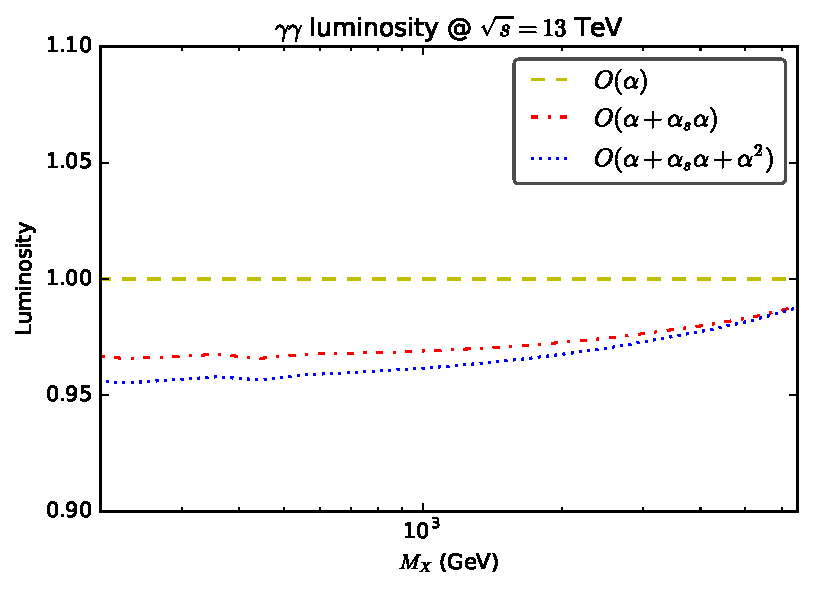
\includegraphics[width=8cm]{figs/lumi_13tev.pdf} 
\caption{$\gamma\gamma$ lunimosity at $\sqrt{s} = 13$ TeV as a
  function of the final state invariant mass $M_X$.}
\label{fig:GammaGammaLumi}
\end{figure}
%%%%%%%%%%%%%%%%%%%%%%%%%%%%%%%%%%%%%%%%%%%%%%%%%%%%%%%%

Fig.~\ref{fig:GammaGammaLumi} shows the behaviour of
$\Phi_{\gamma\gamma}$ computed using the photon PDF $\gamma$ of the
{\tt NNPDF30\_nlo\_as\_0118} PDF set evolved from $Q_0 = 1$ GeV to
$M_X$ including, on top of the pure QCD NLO evolution: only the LO QED
corrections $\mathcal{O}(\alpha)$ (yellow curve), also the mixed
corrections $\mathcal{O}(\alpha_s\alpha)$ (red curve), the full NLO
QCD+QED corrections, $i.e$
$\mathcal{O}(\alpha+\alpha_s\alpha+\alpha^2)$, (blue curve). All
predictions are normalized to the yellow curve. The
$\mathcal{O}(\alpha_s\alpha)$ and $\mathcal{O}(\alpha^2)$ corrections
have a small but non-negligible impact on the
$\gamma\gamma$-luminosity. In particular, these corrections suppress
$\Phi_{\gamma\gamma}$ by almost 5\% at relatively small values of
$M_X$, while the suppression gradually shrinks to 1-2\% as $M_X$
increases. As expected, most of the effect is ascribable to the
$\mathcal{O}(\alpha_s\alpha)$ corrections, while the
$\mathcal{O}(\alpha^2)$ ones have a substatially smaller impact.

\subsection{DIS structure functions}

When considering NLO QCD+QED corrections to the DIS structure
functions, one has to include into the hard cross sections all the
$\mathcal{O}(\alpha)$ diagrams where one photon is either in the
initial state or emitted from an incoming quark (or possibly an
incoming lepton). Such diagrams are of purely QED origin and no QCD
contributions are present. As a consequence, the corresponding
coefficient functions can easily be derived from the QCD expressions
just by properly adjusting the colour factors. In addition, this
correspondence holds regardless of whether mass effects are included
or not.

The main complication arises from the flavour structure. In fact, due
to the fact that the coupling of the photon is proportional to the
squared charge of the parton to which it couples (a quark or a
lepton), in the case of quarks the isospin symmetry is broken.











\end{widetext}